\documentclass[a4paper,12pt,oneside]{article}
\usepackage[T1]{fontenc}
\input{glyphtounicode}
\pdfgentounicode=1
\usepackage[margin=2.5cm]{geometry}
\usepackage{graphicx}
\usepackage{amsmath,amssymb,mathtools}
\usepackage{booktabs}
\usepackage{microtype}
\usepackage{setspace}
\usepackage{etoolbox}
\usepackage{caption}
\usepackage{algorithm}
\usepackage{algpseudocode}
\usepackage{placeins}
\usepackage{xcolor}
\usepackage{tikz}
\usepackage{url}
\usepackage[hidelinks,unicode]{hyperref}
\graphicspath{{figures/}{assets/}}
\setstretch{1.15}
\setlength{\parindent}{1.5em}
\setlength{\parskip}{0.15em}
\captionsetup{font=small,labelfont=bf}
% Keep dedicated float pages compact and aligned to the top, rather than
% distributing large vertical gaps between a table and a figure.
\makeatletter
\setlength{\@fptop}{0pt}
\setlength{\@fpsep}{20pt}
\setlength{\@fpbot}{0pt plus 1fil}
\AtBeginDocument{\typeout{REPORT-FORMAT: font=\f@size pt; textwidth=\the\textwidth; textheight=\the\textheight}}
\makeatother
\newcommand{\astar}{A\ensuremath{^*}}
\newcommand{\source}[1]{\path{#1}}
% Cover information supplied by the project group.
\newcommand{\ReportAuthor}{Nguyen Hoang Thang}
\newcommand{\ReportAuthorsPDF}{Nguyễn Đức Hòa, Phạm Văn Bảo Phong, Nguyễn Bá Hoàng, Nguyễn Hoàng Thắng, Nguyễn Hưng Phát}
\newcommand{\ReportUniversity}{HCMC UNIVERSITY OF TECHNOLOGY}
\newcommand{\ReportFaculty}{FACULTY OF APPLIED SCIENCE}
\newcommand{\ReportLogoPath}{assets/hcmut-logo.png}
\newcommand{\ReportLecturer}{Phan Thanh An}
\newcommand{\ReportClass}{CC06}
\newcommand{\ReportStudentRows}{%
Nguyễn Đức Hòa & CC06 & 2652600 \\
Phạm Văn Bảo Phong & CC06 & 2652465 \\
Nguyễn Bá Hoàng & CC06 & 2651237 \\
Nguyễn Hoàng Thắng & CC06 & 2550216 \\
Nguyễn Hưng Phát & CC06 & 2651590 \\
}

\hypersetup{pdftitle={A* Search Algorithm: Road Routing and Partially Observed Robot Navigation},pdfauthor={\ReportAuthor}}
\begin{document}
\raggedbottom
\hypersetup{pageanchor=false}
\begin{titlepage}
\thispagestyle{empty}
\begin{tikzpicture}[remember picture,overlay]
  \foreach \inset in {1.0,1.15,1.3} {
    \draw[line width=0.5pt]
      ([xshift=\inset cm,yshift=-\inset cm]current page.north west)
      rectangle
      ([xshift=-\inset cm,yshift=\inset cm]current page.south east);
  }
\end{tikzpicture}
\begin{center}
{\small\bfseries \ReportUniversitySystem\par}
\vspace{0.3cm}
{\large\bfseries \ReportUniversity\par}
\vspace{0.3cm}
{\small\bfseries \ReportFaculty\par}
\vspace{1.4cm}
\IfFileExists{\ReportLogoPath}{%
  \includegraphics[width=3.4cm,height=3.4cm,keepaspectratio]{\ReportLogoPath}%
}{%
  \fbox{\parbox[c][3.2cm][c]{3.2cm}{\centering\small\color{gray}Official HCMUT logo\\to be supplied}}%
}
\vspace{1.4cm}
\par{\Large\bfseries PROJECT REPORT\par}
\vspace{0.9cm}
{\Huge\bfseries A* SEARCH ALGORITHM\par}
\vspace{0.8cm}
{\large\bfseries Road Routing and Partially Observed\\Robot Navigation\par}
\vspace{0.4cm}
{\large Design, Implementation, and\\Experimental Evaluation\par}
\vfill
{\large Author: \textbf{\ReportAuthor}\par}
\end{center}
% Blank optional fields print nothing; enter approved values in metadata.tex.
\newcommand{\OptionalCoverField}[2]{\ifdefempty{#2}{}{\par\noindent #1: #2}}
\OptionalCoverField{Course}{\ReportCourse}
\OptionalCoverField{Lecturer}{\ReportLecturer}
\OptionalCoverField{Student ID}{\ReportStudentID}
\OptionalCoverField{Class}{\ReportClass}
\OptionalCoverField{Submission date}{\ReportSubmissionDate}
\vspace{1cm}
\end{titlepage}

\pagenumbering{roman}
\hypersetup{pageanchor=true}
\section*{Abstract}
\addcontentsline{toc}{section}{Abstract}
Heuristic search solves known shortest-path problems while remaining one component of navigation in unknown environments. This report presents reusable C++17 A* integrated with directed road routing and partially observed robot navigation. The robot accumulates limited-range observations, selects exploration targets, repeatedly plans on a verified visibility graph, and returns to observed ancestors. Recorded reversible entry motion bounds executed retreat under explicit assumptions. Evaluation uses a frozen benchmark. On 180 directed road queries, A* and Dijkstra return equal costs; A* reduces expansions by a median paired 76.0\% and has a median search-time ratio of 0.338. A separate comparison retains 21 nontrivial local requests from 351 source decisions. The original authors' approximate-path procedure and our A* adapter both produce obstacle-interior-valid point paths in every retained request, with zero median paired length difference. Different graphs, boundary conventions, and timing stages limit stronger comparisons. Supporting studies examine exploration, sensing, frontier caching, and certified returns. The implementation provides a reproducible case study of graph-optimal planning and conditional recovery under partial observability.

\noindent\textbf{Keywords:} A* search ; Road routing ; Partial observability ; Visibility graph ; Blind-alley recovery ; Reproducible evaluation

\clearpage
\begingroup
\setstretch{1}
\setlength{\parskip}{0pt}
\tableofcontents
\endgroup
\clearpage
\pagenumbering{arabic}
\section{Introduction}
The information available to a planner determines which paths it can evaluate and optimize. Known road topology and edge costs define a fixed optimization problem. A robot with limited vision must also choose where to obtain observations before planning through unknown passages. A locally optimal path may lead into a dead end, requiring return to an observed branching position. Graph search and exploration therefore address distinct, related problems.

This project investigates one C++ implementation of \astar{} in both settings. Road Navigation minimizes distance on a static directed graph. Blind-Alley Robot Navigation plans continuous piecewise-linear motion between exploration targets and returns to observed ancestors using accumulated polygonal observations. Python supplies sensing and exploration around the shared engine. An educational Robot Lab and four-direction blind-alley fixtures remain validated baselines.

Phan et al.~\cite{phan2026} investigate navigation through blind-alley regions and analyze return-path properties under stated geometric assumptions. Their method represents explored space through bundles of line segments and refines paths geometrically. Here, recorded reversible motion supplies a feasible return while \astar{} seeks a shorter verified graph path. This alternative requires explicit sensing and execution assumptions. Comparison must also distinguish computed approximate paths from recorded simulator coordinate transitions.

Accordingly, we examine three questions: how adapters preserve search assumptions; what effort and time geographic guidance saves relative to Dijkstra on the same road graph; and how local robot paths differ at identical observed states and endpoints. The last comparison accounts for representation, validity conventions, and computation stages. Separate online studies examine exploration ordering and executed recovery.

The contribution is a reproducible implementation and controlled evaluation of shared graph search, together with a conditional executed-return certificate. Its scope is established \astar{} theory and observed-graph planning; global unknown-world optimality is not established. Measurements use frozen revision \source{04c4846}.

The report proceeds from theoretical foundations and the problem formulation to system architecture and implementation. The methodology and results distinguish fixed-road shortest paths, shared-state local robot planning, and supporting online behavior. The final sections state limitations, future improvements, and the project conclusions.

\section{Theoretical Foundation and Literature Review}
\subsection{Shortest-Path Search and Heuristic Assumptions}
Once a graph is available, both applications require minimum-cost paths. On directed $G=(V,E,w)$ with nonnegative weights, Dijkstra orders pending states by tentative start cost~\cite{dijkstra1959}. \astar{} adds estimated remaining cost to guide search toward the goal~\cite{hart1968}:
\begin{equation}f(n)=g(n)+h(n).
\end{equation}
Here $g(n)$ is the best start-to-$n$ cost found so far and $h(n)$ estimates cost to goal $t$. OPEN contains pending states; improvements update costs and predecessors. The goal is accepted on valid minimum-priority extraction, not discovery. Setting $h=0$ gives Dijkstra in the same implementation.

This stopping rule requires suitable estimates. Admissibility means $0\leq h(n)\leq h^*(n)$, where $h^*(n)$ is minimum remaining graph cost. Consistency additionally requires
\begin{equation}
h(u)\leq w(u,v)+h(v)\quad\text{for every }(u,v)\in E,\qquad h(t)=0.
\label{eq:consistency}
\end{equation}
Consistency makes the first valid expansion's cost optimal. Admissible but inconsistent estimates can require reopening improved states. These distinctions and tie resolution underlie Hart et al.~\cite{hart1968} and the implementation in Section~5. Fewer expansions need not mean lower wall time: heuristic evaluation and representation also incur work.

\subsection{Geometric Representation and Replanning}
Optimality depends on admitted paths. Grids restrict headings and may miss narrow passages; visibility-based planning uses obstacle-free geometric connections~\cite{lozano1979}. Finite footprints require configuration-space treatment. A complete polygonal visibility graph and a sparse scan-center graph admit different paths, so optimality in the latter need not imply a continuous shortest path.

Theta* uses grid search with off-grid connections~\cite{daniel2010}. Experiments on random grids and game maps compare length, time, expansions, and heading changes, finding shorter paths than grid smoothing without a full visibility graph. Basic Theta* nevertheless does not guarantee a continuous shortest path. Our ordinary A* on verified continuous links likewise requires separate assessment of representation and search.

When observations change, D* Lite reuses search information through locally consistent value updates~\cite{koenig2002}. Its unknown-terrain navigation and mapping experiments reduce operations relative to repeated search. Those grids initially allow unknown traversal optimistically; our graph admits only verified free links. Repeated A* preserves implementation transparency. Incremental replanning remains an alternative whose project performance is unmeasured.

\subsection{Observation, Exploration, and Escape}
Constructing links first requires representing sensor knowledge. Elfes accumulates uncertain evidence in probabilistic occupancy grids~\cite{elfes1989}; sonar and stereo demonstrations show the value of additional viewpoints. Our deterministic labels and polygon unions accumulate observations and preserve unknown space, but omit probabilistic uncertainty and localization drift.

Free/unknown boundaries then suggest exploration targets. Yamauchi visits accessible frontiers~\cite{yamauchi1997}; office-robot experiments address sensor artifacts, while idealized coverage remains conditional on sensing and reachability. Our polygon candidates similarly seek observations, using ancestry for recovery and C++ A* for routing. Estimated utility does not prove information gain, and one unreachable candidate does not exhaust a branch.

TangentBug combines range discontinuities and a local tangent graph with target motion and boundary following~\cite{kamon1996}. Its convergence analysis assumes static finite-perimeter geometry and ideal point motion; selected simulations compare it with VisBug. Our simpler observed-parent policy does not inherit that guarantee. Together these studies explain why local path optimality requires a separate exploration and escape mechanism.

\subsection{Bundle-Based Planning and the Assigned BAR Problem}
Phan et al.~\cite{phan2026} accumulate sights, rank active open points, construct a skeleton graph, and shorten polylines through ordered bundles of line segments. DAP adjusts vertices on critical segments within represented explored space; Section 3 relates approximation quality to geometric and numerical assumptions. Section 4.5 constructs bundles and Algorithm 2 integrates observations, ranking, refinement, and movement. The main contribution is geometric representation and refinement, not ordinary graph search.

Algorithm 2 is explicitly not generally convergent. Section 5 studies a special algorithm with obstacle-diameter and near-goal connectivity assumptions, which do not prove completion of our maze exploration. Section 6 compares local paths with a grid A* baseline and RRT*, and further evaluates RRTX. Dijkstra is discussed as a foundational search method rather than evaluated as an independent experimental baseline. The source's \source{Graph.BFS_skeleton_path} performs Dijkstra-style cumulative-cost priority-queue search, despite its BFS-oriented name; this skeleton search precedes bundle-based refinement.

These differences determine the scope of our comparison: observations and endpoints are held fixed, while graph representations, boundary rules, and motion semantics are disclosed. The application addresses exploration with limited sensing and conditionally certified return to observed ancestors. It reproduces neither bundle optimization nor general polygonal BAR detection. The supplementary literature matrix records the relevance of all eight supplied PDFs, representing seven unique studies.

\section{Problem Formulation}
\subsection{Known Directed Road Routing}
Let $G=(V,E,w)$ be a finite directed road graph with finite nonnegative weights $w:E\to\mathbb{R}_{\geq0}$. For origin $s\in V$ and destination $t\in V$, the routing objective is
\begingroup\predisplaypenalty=0
\begin{equation}
P^*\in\underset{P:s\leadsto t}{\operatorname{argmin}}\;
C(P),\quad C(P)=\sum_{(u,v)\in P}w(u,v).
\end{equation}
\endgroup
Here $C(P)$ sums exported road lengths in meters. Directed edges enforce one-way topology; traffic, time-dependent costs, and turn restrictions absent from preprocessing are excluded. If no path exists, search reports failure. Node endpoints isolate search from coordinate snapping in the principal experiment. Interactive requests instead use projected road positions and temporary partial edges (Section~4).

\subsection{Partially Observed Robot Navigation}
Let $W\subset\mathbb{R}^2$ be a bounded workspace and $O\subset W$ the static polygonal obstacles. At controller decision $k$, define robot position $x_k$, goal $q$, accumulated observed free space $F_k$, and visible obstacle fragments $B_k$. The simulator uses $O$ for sensing and motion validation; the policy receives observed geometry and traversal history. Its unknown region is $U_k=W\setminus(F_k\cup B_k)$. Range $R>0$ and occlusion limit observations: membership in the sensing disk alone establishes neither visibility nor traversability.

The controller selects target $z_k$ from observed information and history, then constructs $G_k=(V_k,E_k)$ from scan centers and request endpoints. Only wholly verified free segments become links. Edge weights $\|u-v\|_2$ and heuristic $\|u-z_k\|_2$ let \astar{} minimize graph-path length. Execution checks collision and observed-free coverage. For consecutive executed positions $y_0,\ldots,y_M$, the complete journey has length
\begin{equation}
L_{\mathrm{online}}=\sum_{j=0}^{M-1}\|y_{j+1}-y_j\|_2.
\end{equation}
This quantity includes both exploration and return motion. The index $j$ counts executed segments, whereas $k$ counts controller decisions; neither counts rendered frames. Consequently, $L_{\mathrm{online}}$ need not equal one local plan's cost or the shortest distance available with full-map knowledge.

The continuous simulator uses an idealized point center and reversible motion along straight segments. Heading changes freely at vertices; acceleration, nonholonomic constraints, and disk clearance are absent. The frozen local comparison permits boundary tangency in its primary convention and separately reports strict no-contact validity. Neither convention validates the source's nominal radius-0.5 parameter.

\subsection{Recovery and Evaluation Objectives}
A branch records an observed anchor and its subsequent executed trajectory. Exhaustion of usable local candidates triggers return to an observed ancestor with remaining alternatives. Failure to reach one target instead defers it for reconsideration after knowledge changes; it does not certify branch exhaustion. Exploration resumes after return. Section~5 derives the conditional executed-length bound.

Road evaluation measures minimum graph cost, valid expansions, and search-call time. Local robot evaluation measures planned Euclidean length, geometric turns, endpoint agreement, observed-space coverage, obstacle validity, and computation components. Supporting online studies measure actual distance, goal status, frontier processing, and executed returns. A return to an observed ancestor is \emph{certified} only when the recorded entry trajectory is reversible and the executed return satisfies the prescribed endpoint and length constraints. Reaching a goal, ending with no eligible frontier, and exhausting a budget are different outcomes; none automatically proves a complete map or global unknown-world optimality.

\section{System Architecture and Design}
\subsection{Shared Engine and Application Boundaries}
Figure~\ref{fig:architecture} separates shared search from application knowledge. React/TypeScript requests pass through FastAPI and pybind11 to C++17. Road loading and adapters are C++; Python handles continuous sensing, accumulated geometry, targets, ancestry, and execution. Python constructs the continuous graph; the binding validates points and links and assigns Euclidean costs. Search therefore needs no hidden obstacle geometry.

\begin{figure}[!htbp]
\centering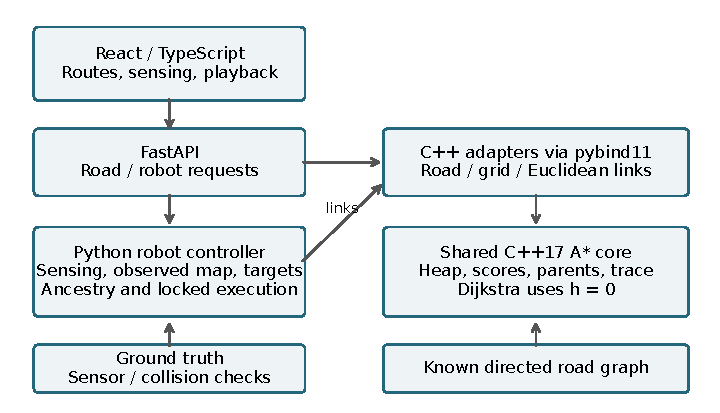
\includegraphics[width=0.8\textwidth]{architecture.pdf}
\caption{Implemented system boundaries. Ground truth enters sensing and motion validation; the continuous planner receives observations and verified links. Traces support frontend playback.}
\label{fig:architecture}
\end{figure}

Reuse requires a common problem contract. \source{include/astar/search.hpp} accepts neighbors, heuristic, goal predicate, and state hashing/equality, maintaining costs, predecessors, counters, and traces without coordinate or equal-cost assumptions. Disabling the heuristic gives Dijkstra in the same core, isolating guidance in the road comparison.

\subsection{Road Representation and Coordinate Requests}
The OSM-derived graph contains 2,986 vertices and 7,152 directed edges. Adjacency determines legal travel; polyline metadata supplies geometry (Fig.~\ref{fig:roads}). Snapping a click between intersections to a vertex would shift the endpoint. Queries instead scan segments and project using latitude-scaled coordinates. Cumulative Haversine lengths determine edge fraction $r\in[0,1]$; projection remains a local approximation.

\begin{samepage}
For directed edge $u\rightarrow v$ of weight $w$, a snapped start connects forward with $(1-r)w$, and a snapped goal connects from $u$ with $rw$. Reverse travel requires a corresponding reversed polyline and uses its own weight and fraction. Two ordered positions on one directed edge obtain a direct connection of $(r_g-r_s)w$ when $r_g\geq r_s$. Endpoints reuse real nodes. Virtual states and partial edges belong only to the request adapter; the base graph is unchanged. Partial route geometry is sliced along the original polyline. The heuristic scale is also reduced if a partial edge requires it. Thus floating-point or geometric approximations do not justify blindly reusing an invalid lower bound.
\par\end{samepage}

\begin{figure}[!htbp]
\centering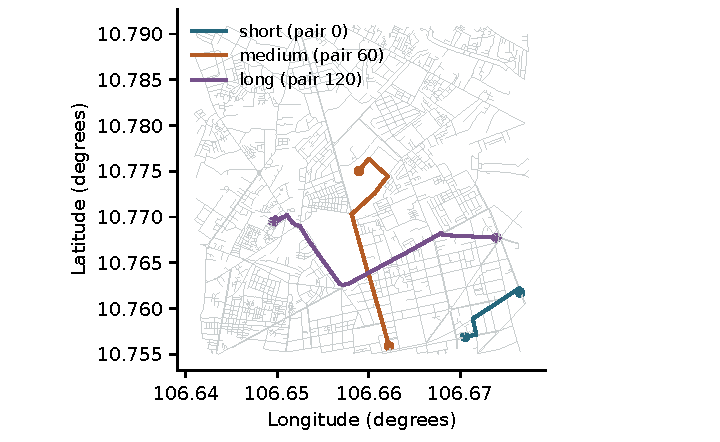
\includegraphics[width=\textwidth]{roads.pdf}
\caption{Representative frozen short, medium, and long road queries. Background is the exported graph, not additional routing information; each highlighted route uses the unchanged C++ adapter. Axes use exported geographic coordinates.}
\label{fig:roads}
\end{figure}

\subsection{Sensing, Exploration, and Observed Ancestry}
Robot Lab supports four or eight directions (diagonal cost 1.5, without corner cutting), and grid BAR uses four unit-cost directions. Continuous polygon, seeded-maze, and indoor modes admit arbitrary straight-link headings, but require conservative observation geometry.

The sensor uses 72 uniform directions and rays near visible vertices. First-hit range, blocker margins, and checked free triangles approximate visibility before union into $F_k$. Occlusion distinguishes this region from the sensing disk. The policy receives observations without hidden polygons or topology; grid evaluation gates are consulted only after navigation. Ground-truth annotations are used only for evaluation and do not influence target selection or recovery decisions.

\begin{samepage}
Traversal history enables recovery. Each exploration node records position, history index, branch ID, parent ID, and remaining candidates; a stack tracks ancestry. Rounded target identities prevent immediate repetition, while map or observation changes permit reconsidering deferred targets. Radar ranking estimates frontier opportunity from known boundaries and discounts direct Euclidean travel. This proxy is neither a C++ \astar{} path cost nor guaranteed information gain. Low gain does not exhaust a branch; a conservative fallback retains uncertain occluded candidates.
\par\end{samepage}

Recovery transfers deferred child alternatives, preserves siblings, and locks execution to the anchor. Graph-blocked targets remain distinct from exhausted branches. Playback displays sensing, plans, movement, branches, and returns, with graph debugging hidden by default. Search traces expose $g,h,f$ and predecessors; continuous frames describe higher-level events. Display interpolation introduces no executed motion.

From the user's perspective, both applications submit a planning request and display its returned path and trace. The interfaces share a search engine but provide different problem adapters: road requests supply a known directed network, while robot requests operate on accumulated observed geometry. Python manages sensing and exploration; the C++ engine evaluates the verified graph supplied to it. This separation makes the implementation reusable without exposing hidden obstacles to the robot planner.

\section{Algorithm Implementation}
\subsection{Queue, Records, and Improved Paths}
Preserving improvements to pending or expanded states requires separating records from queue entries. An \source{unordered_map} stores best $g$, predecessor, and last-expanded $g$ per state; a \source{priority_queue} stores state, inserted $g,h,f$, and insertion order. Lexicographic $(f,h,\mathrm{order})$ selects lower $f$, lower $h$, then earlier insertion, deterministically when neighbor enumeration is deterministic.

\begin{samepage}
Algorithm~\ref{alg:core} pushes a new entry for each improvement rather than decreasing a key. Entries with stored $g$ above the current best record, or no better than the last-expanded score, are skipped. The last-expanded $g$-score records expansion history without permanently closing a state, thereby allowing reopening when a strictly better path is found.
\par\end{samepage}

\begin{algorithm}[H]
\caption{Shared C++ search (trace and counters omitted)}\label{alg:core}
\begin{algorithmic}[1]
\Require Problem neighbors, heuristic, goal predicate; start $s$, goal $t$
\State Initialize records with $g=\infty$, no parent or expanded value
\State $g[s]\gets0$; push $(s,0,h(s),h(s),\mathrm{order}{+}{+})$
\While{OPEN is not empty}
  \State Pop minimum entry $e$ with state $u$
  \If{$e.g>g[u]$ or ($u$ expanded and $e.g\geq g_{\rm expanded}[u]$)}
    \State \textbf{continue}
  \EndIf
  \State $g_{\rm expanded}[u]\gets e.g$
  \If{problem goal predicate holds for $u,t$}
    \State \Return predecessor chain reversed, cost $e.g$
  \EndIf
  \For{outgoing $(u,v,w)$}
    \State Validate finite $w\geq0$; $a\gets e.g+w$
    \If{$a<g[v]$}
      \State $g[v]\gets a$; parent$[v]\gets u$
      \State Validate $h(v)$ and finite sum; push $(v,a,h(v),a+h(v),\mathrm{order}{+}{+})$
    \EndIf
  \EndFor
\EndWhile
\State \Return not found, empty path, infinite internal cost
\end{algorithmic}
\end{algorithm}

The subsequent goal test prevents stale entries from terminating search. Reconstruction follows predecessors to the parentless start and reverses them. Start equals goal yields a zero-cost singleton; failure yields an empty path and internal infinity, serialized as nullable cost. The engine rejects nonfinite or negative weights/estimates and overflow. Relaxation uses strict improvement, with tolerances only in external validation. Adapters remain responsible for admissibility.

For a finite graph, consistent heuristic, binary heap, and expected constant hashing time, lazy entries give a conservative $O((|V|+|E|)\log(|V|+|E|))$ time and $O(|V|+|E|)$ auxiliary-space bound. Geometry and traces add costs. Inconsistent estimates may reopen states, invalidating a single-expansion bound.

\subsection{Application Heuristics and Trace Semantics}
Heuristics follow the movement model. For roads, let $d_H$ be Haversine distance in meters. The loader chooses $0\leq\alpha\leq1$ with $\alpha d_H(u,v)\leq w(u,v)$ on every edge and sets $h(u)=\alpha d_H(u,t)$. The spherical triangle inequality gives $h(u)\leq\alpha d_H(u,v)+h(v)\leq w(u,v)+h(v)$, establishing Eq.~\ref{eq:consistency}. The frozen graph retains $\alpha=1$; this bound requires no reverse edges.

For absolute grid differences $dx,dy$, four-direction unit movement uses Manhattan distance; eight-direction Robot Lab uses $\max(dx,dy)+0.5\min(dx,dy)$ for its diagonal cost of 1.5. Euclidean continuous-link weights make Euclidean goal distance consistent by the ordinary triangle inequality. Each guarantee thus concerns the adapter's admitted paths.

Expanded nodes count valid pops, including goal and re-expansions; generated nodes count all pushes. Unique counts are separate. Examined and relaxed edges count scanned neighbors and improvements. Trace events expose discovery, updates, expansion, closure, and goal scores. Stale entries are skipped; timing disables traces.

\subsection{Executed Return Certificate}
Recovery requires an executed-motion bound. Let $T=(a=p_0,\ldots,p_m=b)$ be recorded entry from anchor $a$ to current $b$, with $L_T=\sum_{i=0}^{m-1}\|p_{i+1}-p_i\|_2$. Under static obstacles, sound observed-free checks, and reversible point motion, its reverse is feasible with equal length. If recorded waypoints and links appear in the planning graph, graph-optimal \astar{} gives $L_{A^*}\leq L_T$. Acceptance additionally checks endpoints, segment coverage, and length. Planning failure or an excessive length invokes the separately verified recorded reverse.

To preserve the bound during execution, the controller completes the accepted return without switching to exploration. For measured length $L_R$ and final position $x_{\rm end}$, it requires
\begin{equation}
L_R\leq L_T+\varepsilon,\qquad
\|x_{\rm end}-a\|_2\leq\varepsilon,
\label{eq:return}
\end{equation}
Here $\varepsilon$ represents numerical length and endpoint tolerances in world units. Sensing may add observations without changing the destination. Certification requires verified reversible entry and locked execution; it does not establish semantic BAR boundaries, disk clearance, universal detection, or completeness. Reversed-entry fallback can satisfy the bound without an A*-computed shortcut, so outcomes are recorded separately.

\section{Experimental Methodology}
\subsection{Frozen Inputs and Controlled Road Comparison}
The experiments distinguish heuristic guidance on a fixed graph, local geometry at shared observed states, and online exploration/recovery. Only the first isolates a search algorithm change; the others require representation and execution qualifications. Inputs and results are frozen at \source{04c4846}, with manifest hashes and an unmodified authors' checkout at \source{8bbbfb8}.

The recorded host is Windows 11, Intel Core 7 240H (16 logical processors), with approximately 15.7 GiB RAM. CMake builds C++17 Release using MSYS2 UCRT64 g++; the binding runs in Python 3.12.10, original ASP in Python 3.14.2. Different environments and uncontrolled frequency/load make timings descriptive, not algorithm-only comparisons.

To examine route-length dependence, selection sampled 6,000 directed candidates with seed 20261009; 5,965 were reachable. Dijkstra ranks define strata at approximately 2,086.98 and 3,273.44 m, retaining 60 queries each for 180 frozen benchmark queries.

Only the heuristic flag changes between methods on the same graph and engine. One untimed call precedes seven alternating-order batches of 20, 10, and 5 calls in the respective strata. Time is the median batch mean per call. Loading, snapping, HTTP, rendering, and traces are excluded; common timed status/cost checks remain.

\subsection{Source Audit and Shared-State Robot Requests}
Compatible motion semantics are necessary for end-to-end comparison. The source logs an ASP but updates coordinates to its selected open point without ASP interpolation; Algorithm 2 specifies DAP motion. Straight-chord interpretations produce four interior crossings in the dead-end reproduction and one in the bugtrap, while planned ASPs avoid interiors. Coordinate transitions alone do not establish physical trajectories. The 48-configuration matrix therefore remains blocked and unexecuted: its entries are not failures, and chord distances cannot be compared with our executed travel.

A local comparison avoids inferring motion: requests freeze position, target, sights, skeleton, ASP, and provenance. The original routine is replayed unchanged. Our A* uses identical endpoints and sights, with analytic whole-link certification in a scan-center graph. This adapter preserves circular boundaries rather than the application's polygon approximation. Full polygons enter only post-plan validation, never planner decisions.

Eligibility precedes local outcomes and requires more than two skeleton vertices, selecting nontrivial bundle refinement. Cohorts contain 43, 75, and 233 decisions (Table~\ref{tab:eligibility}). Prospective selection preceded ten episodes at radii 10/20/30, capped at 60 iterations; capped outcomes remain. Correlated decisions and overlapping prior held-out bugtrap geometry limit generalization.

\begin{table}[htbp]
\caption{Frozen robot decision accounting. Direct exclusions do not invoke bundle refinement; they are retained in the raw audit.}\label{tab:eligibility}
\centering\begin{tabular}{lrrr}\toprule
Cohort & Captured & Eligible & Excluded\\\midrule
Initial &43&6&37\\
Prior held-out &75&1&74\\
Prospective extension &233&14&219\\\midrule
Combined &351&21&330\\\bottomrule
\end{tabular}
\end{table}

\begin{samepage}
Direct exclusions comprise 176 source-visible and 154 strict-range-boundary cases. Boundary convention explains endpoint predicate differences, with no missing-input or eligibility-checker mismatch. All 21 eligible requests remain, regardless of planner outcome.
\par\end{samepage}

\subsection{Validity, Metrics, and Timing Boundaries}
Primary robot validity requires matching endpoints within $10^{-7}$, full observed-sight segment coverage, and no polygon-interior entry; boundary contact is permitted. Strict point validity rejects boundary contacts as well. Radius-0.5 clearance is a separate offline diagnostic, not the planned collision model. Event-based segment certification uses tolerance $10^{-9}$; sampled predicate comparisons supplement it rather than prove universal sensor equivalence. Across all cohorts, 175,500 membership samples and 111,672 graph-link samples have no unexplained mismatch or uncovered sample. All 865 recorded ASP segments are sight-certified; 1,128 accepted A* graph links avoid polygon interiors and boundaries offline.

Length is a sum of Euclidean polyline segments. An all-turn count uses wrapped heading changes exceeding $10^{-6}$ radians; an interpretable significant-turn count uses changes greater than $15^\circ$. Neither is a motor command count. ASP critical-line counts and A* expansions are not interchangeable operations. Robot component timing uses three warm-ups and 31 measured calls per state, then medians across state medians. ASP core excludes source skeleton generation; A* graph construction includes observed-link certification and is separated from its binding/search call. Medians of components need not sum to a median pipeline time.

Separate online studies retain 20 legacy/radar pairs, 20 full/cached frontier pairs, 12 sensor episodes, and an indoor parent trace. They measure our executed behavior, not local planning against the authors. Statistics are paired by configuration before aggregation, without significance or population-superiority claims. Report scripts leave frozen results unchanged.

\section{Results and Discussion}
\subsection{Road Cost Agreement and Search Effort}
All 180 matched road queries return equal costs under A*, Dijkstra, and the frozen offline reference within $10^{-6}$ m. The graph validator reports zero heuristic edge violations and scale 1.0. Separately retained edge cases cover start equals goal, unreachable targets, directionality, and edge-midpoint snapping. These checks support correctness on the tested graph; agreement alone is not a proof for every possible adapter.

\begin{table}[!htbp]
\caption{Frozen road results; 60 pairs per stratum. Expansion and time columns are marginal medians; reduction and ratio are medians of paired statistics.}\label{tab:road}
\centering\begin{tabular}{lrrrr}\toprule
Stratum & Expanded A*/D & Reduction & Time A*/D ($\mu$s) & Ratio\\\midrule
Short &101 / 505&78.6\%&44.95 / 128.09&0.324\\
Medium &301 / 1,592&77.4\%&282.95 / 1,117.24&0.287\\
Long &714.5 / 2,588.5&68.6\%&771.46 / 1,883.19&0.449\\\bottomrule
\end{tabular}
\end{table}

\begin{figure}[!htbp]
\centering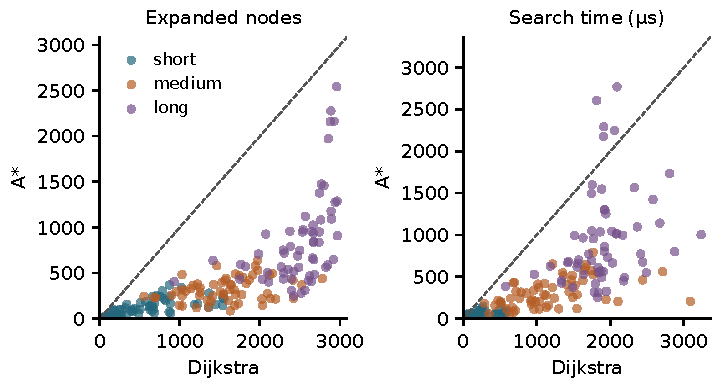
\includegraphics[width=\textwidth]{road-effort.pdf}
\caption{Matched road search effort and search-call timing. Points below the diagonal favor A*. Each stratum has 60 queries; all 180 costs agree. Timing excludes graph loading, snapping, API, and rendering.}
\label{fig:road-effort}
\end{figure}

\begin{samepage}
Table~\ref{tab:road} and Fig.~\ref{fig:road-effort} show fewer expansions in every A* run, with median paired reduction 76.0\%. Geographic guidance directs search toward the destination while preserving the cost objective. A* is faster in 173 cases, Dijkstra in seven; the median paired time ratio is 0.338, range 0.061--1.435, with pair 167 the largest regression. These data support substantial savings on this network, not universal timing dominance. Paired ratios differ from ratios of marginal medians. The shared graph controls representation more tightly than the robot study.
\par\end{samepage}

\subsection{Robot Local Geometry and Path Length}
Both local planners find paths for all 21 eligible requests, with correct endpoints and primary interior-only validity in all 21. These are local planning successes, not 21 successful autonomous missions. Of the ten prospective source episodes, nine reach the goal and one reaches its iteration cap; its eligible states remain. Figure~\ref{fig:observed} shows an observed-space request and the two returned paths. No hidden polygons are supplied to either local planner.

\begin{table}[htbp]
\caption{Local robot outcomes by cohort. ``Shorter'' counts follow the primary point convention. Two prospective cases have equal lengths. Delta is the median paired A* minus ASP length in world units.}\label{tab:robot}
\centering\begin{tabular}{lrrrr}\toprule
Cohort &Pairs&ASP shorter&A* shorter&Delta\\\midrule
Initial &6&5&1&$+7.403$\\
Prior held-out &1&1&0&$+1.654$\\
Prospective &14&3&9&$-2.492$\\\midrule
Combined &21&9&10&$0.000$\\\bottomrule
\end{tabular}
\end{table}

\begin{figure}[!htbp]
\centering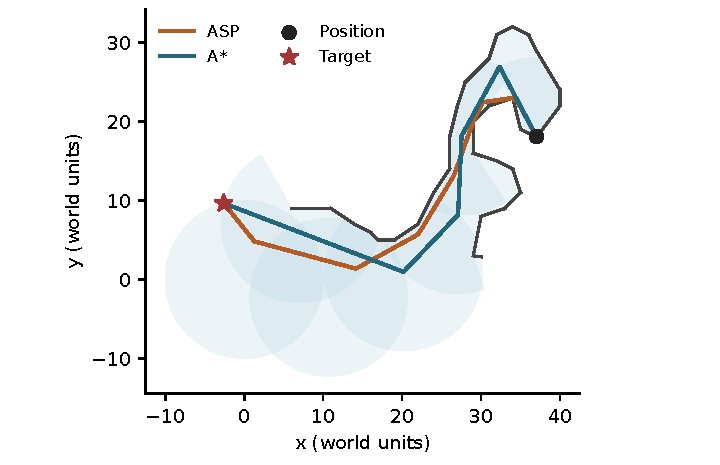
\includegraphics[width=\textwidth]{robot-observed.pdf}
\caption{Representative frozen dead-end request. Visible blocker fragments and approximate display sight footprints show recorded knowledge; ASP and scan-center A* use the same position and target. Sight footprints are display approximations; benchmark link admission uses analytic whole-segment certification. Hidden obstacles are omitted.}
\label{fig:observed}
\end{figure}

\begin{samepage}
Define paired difference as A* length minus ASP length; positive values favor ASP. ASP is shorter in nine requests, A* in ten, and two are equal. The median is zero, mean $+2.981$, and range $[-10.707,+44.266]$ world units. Different representations admit different paths, and neither planner consistently dominates. Cohort composition matters: five of six initial cases favor ASP, nine of fourteen prospective cases favor A*. Figure~\ref{fig:robot-length} retains all pairs; one held-out request cannot establish generalization.
\par\end{samepage}

\begin{figure}[!htbp]
\centering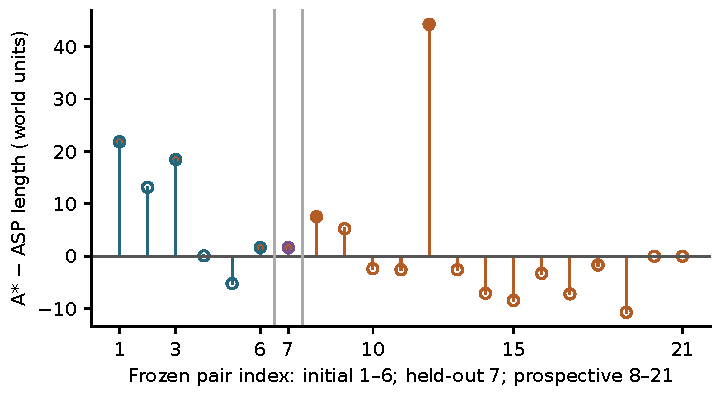
\includegraphics[width=\textwidth]{robot-length.pdf}
\caption{All 21 eligible local requests, grouped by frozen cohort. Positive A* minus ASP differences favor ASP. Filled orange markers indicate ASP boundary contact under the strict convention; these paths remain primary interior-valid.}
\label{fig:robot-length}
\end{figure}

Boundary conventions explain part of this variation. ASP passes strict validity in 15 of 21 requests and A* in all 21. All six boundary-touching ASP paths are shorter under the permissive convention. A dead-end configuration with the largest difference (\source{P02-_map_deadend-01}) yields 15.734 units for ASP versus 60.000 for A*, with ASP boundary contact. Among 15 jointly strict-valid pairs, ASP is shorter in three, A* in ten, and two tie; median difference is $-2.584$. This secondary criterion cannot replace the primary result. Geometric refinement and strict sparse-center links admit different routes, requiring joint interpretation of length and validity.

Radius-0.5 clearance passes only nine ASP and eleven A* paths, precluding disk-safety claims. Significant-turn medians are two and one respectively; paired all-turn delta median is $-2$. Tiny ASP bends can inflate all-turn counts without corresponding physical steering. ASP vertices can lie inside bundles absent from the sparse A* graph, so mixed lengths do not contradict graph-optimal search.

\begin{figure}[!htbp]
\centering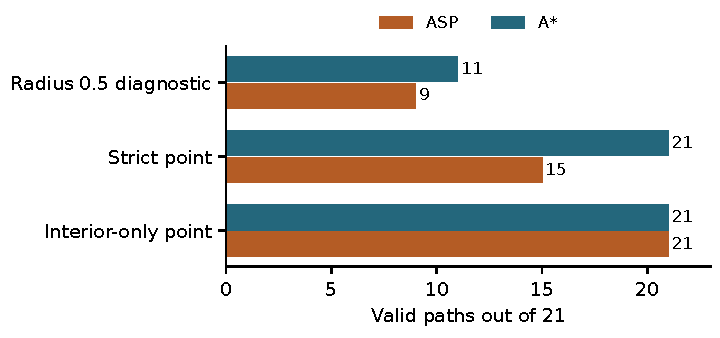
\includegraphics[width=\textwidth]{robot-validity.pdf}
\caption{Validity outcomes for the same 21 requests. Primary point validity allows boundary tangency; strict validity forbids it. Disk clearance is only a post-plan sensitivity check, not a guarantee of executed finite-robot motion.}
\label{fig:validity}
\end{figure}

\subsection{Robot Computation Components}
Figure~\ref{fig:runtime} separates the measured components. Across state medians, ASP core time is 62.655 ms, critical-line construction 0.319 ms, and optimization 62.400 ms. A* link-build time is 42.102 ms, binding/search 0.0263 ms, and the median per-state build-plus-call sum 42.142 ms. The small C++ call is a search on already constructed sparse graphs, while Python geometric certification can dominate its surrounding pipeline.

\begin{figure}[!htbp]
\centering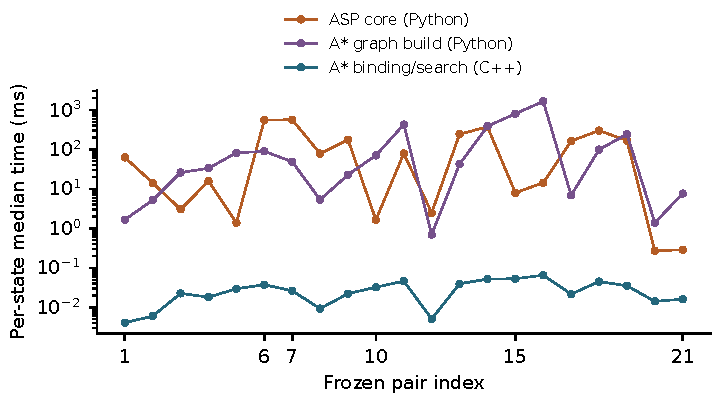
\includegraphics[width=\textwidth]{robot-runtime.pdf}
\caption{Per-state median local computation times (three warm-ups, 31 calls). A logarithmic axis exposes component scale. ASP core excludes skeleton generation; A* build includes observed-link certification. Components and languages differ, so isolated search ratios are not algorithm-only speedups.}
\label{fig:runtime}
\end{figure}

Construction and certification dominate the small C++ call in these requests. Dividing ASP core time by that call would compare different languages and preparation; even build-plus-call and ASP core omit different upstream work. Thus the evidence locates computational cost without isolating intrinsic algorithm speedup. Stronger timing conclusions require matched pipelines.

\subsection{Supporting Online Behavior and Recovery}
Online navigation adds target ordering. Both legacy and radar reach the goal in 20 paired episodes; radar travels less in 18 and more in two, with median difference $-95.419$ world units. Its largest regression is $+70.772$ in Complex Irregular Labyrinth at radius 7. Estimated information changes branch ordering, with useful but non-dominating outcomes; low scores cannot justify exhaustion. All twelve sensor episodes reach their goals, but radius-5 and radius-7 distance medians are 92.909 and 113.278 units. Greater range need not shorten travel in this sample because it also changes decisions.

Caching addresses computation without changing exploration ordering. Full and cached construction preserve playback, recovery, status, and distance in all 20 pairs; median accumulated frontier times are 639.166 and 46.723 ms, respectively. These are episode component totals, not end-to-end timings. Avoiding repeated construction explains the reduction, but equivalence requires invalidation when new free geometry or walls change the mask. Evidence supports the tested indoor and maze configurations, not arbitrary geometric updates.

\begin{figure}[!htbp]
\centering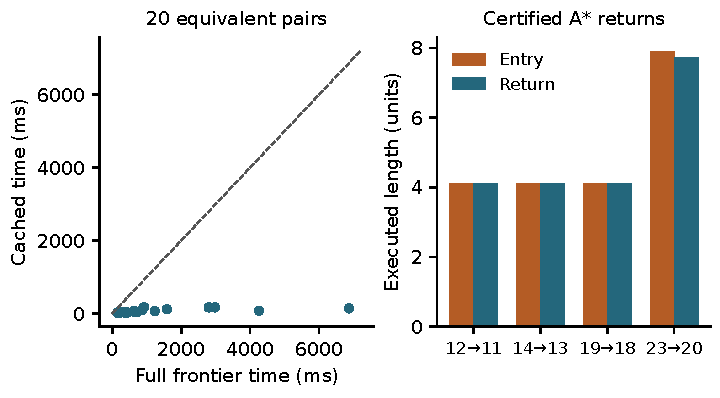
\includegraphics[width=\textwidth]{supporting.pdf}
\caption{Supporting evidence from our online simulator. Left: paired frontier processing with equivalent playback in 20 cases. Right: four observed indoor branch returns, each certified and marked nonfallback in the frozen trace. These are separate from the local authors-versus-A* comparison.}
\label{fig:support}
\end{figure}

The four certified indoor returns in Fig.~\ref{fig:support} are explicitly nonfallback: they demonstrate participation of C++ A* in recovery rather than automatic reversal of entry. Certification checks executed length to the observed ancestor under the assumptions of Eq.~\ref{eq:return}. Successful uncertified exits, unreachable-goal fixtures, and budget termination remain separate outcomes. In particular, a continuous no-frontier status establishes exhaustion of the controller's candidates, not unreachability in the unknown world.

\section{Limitations and Future Improvements}
\paragraph{Model validity.} Static obstacles, ideal localization, reversible point motion, and reliable observations exclude probabilistic sensing, pose drift, dynamics, and footprint-aware configuration space. Sampled sensing may miss narrow occluded regions; accumulated free space differs from the sensing disk. Finite frontier candidates and budgets preclude inferring completeness in arbitrary polygonal worlds from fixture success.

\paragraph{Scope of guarantees.} Missing geometric vertices can make graph-optimal paths longer than continuous optima. The return bound requires verified reversible entry, appropriate endpoints, and locked execution; it proves neither universal BAR identification nor optimal online travel. The paper's approximation and restricted convergence arguments do not transfer to this controller. Our BAR-inspired application retains the stated restrictions rather than reproducing all published mechanisms.

\paragraph{Comparison validity.} Shared observations do not imply shared graphs. Permissive and strict boundaries change interpretation; point validity does not establish disk safety. Source transitions and ASPs do not expose compatible continuous execution, keeping end-to-end comparison gated. Our adapter differs from the paper's grid baseline, so this is not reproduction of its numerical tables. Local timings and selected examples cannot establish superiority.

\paragraph{Sampling and timing.} One road network, convenience robot maps, correlated decisions, overlapping held-out geometry, and 21 eligible requests limit external validity. Prospective selection reduces outcome bias without creating independent random trials. Scheduling, Python versions, compiler settings, batch averaging, and unmatched computation boundaries affect timing. Repetitions and ranges improve auditability without eliminating confounders; paired descriptive results support neither significance claims nor transferable speedup guarantees.

\paragraph{Reproducibility.} Frozen records report four C++ suites, 169 Python tests, 34 frontend tests, and build/lint success, without proving optimal exploration. Report validation checks hashes and statistics without changing results.

\paragraph{Future improvements.} Independent maps and matched computation pipelines would strengthen external validity and timing comparisons. Footprint-aware planning and imperfect sensing require explicit new models and safety checks before any physical-robot claim. Richer geometric vertices or incremental replanning should be evaluated through new controlled experiments; the frozen results do not establish their benefits.

\section{Conclusion}
The information model determines the scope of path optimality. On known directed roads, the shared C++17 A* engine solves a fixed shortest-path problem. Under limited sensing, it solves successive observed-graph problems within an exploration controller. Reversible recorded entry and locked execution conditionally bound returns to observed ancestors, without globally optimizing unknown-world travel.

Road cost agreement accompanies substantial search-effort reductions on the tested network. Shared-state robot paths are primary-valid but have mixed lengths and boundary behavior, precluding general superiority. Timings identify geometric construction costs. Online studies demonstrate cache savings with unchanged tested playback and genuine A*-computed certified returns, while retaining exploration regressions and nonmonotonic sensing outcomes.

The resulting implementation and evaluation provide a reproducible case study of graph search under different assumptions about environmental knowledge. Further work should examine independent maps, footprint-aware geometry, sensing error, and matched pipelines. Incremental replanning or richer geometric vertices require new controlled experiments.

\FloatBarrier
\bibliographystyle{splncs04}
\phantomsection
\addcontentsline{toc}{section}{References}
\bibliography{references}
\end{document}
